\chapter{Analysis}
		For the previous simulations the parameters of every driver were arbitrary chosen. The only constraint was that all of the parameters must be in the range of real values. However it could important that which parameters matter more and which less.
	\section{Effect of the parameters of drivers}
		So all of the important parameters and their effects on the traffic flow should be examined. The tested parameters are the followings: $a_{\rm max}$, $T$ $h_0$ $t_{\rm change} $, $\Delta a_{\rm th}$.
		\subsection{Changing parameters of case 1}
		Let us start with case 1. First increase the parameters by 25 \%. The effect can be seen in Table \ref{tab:vehicle_density_par_pos_case_1} and Figure \ref{fig:vehicle_density_par_pos_case_1}. The original elapsed time is denoted by $t_0$. As the result shows $\amax$ has the greatest improvement on time however it is still not significant. The greatest regression comes with $T$, the safe headway time. The effect of the other parameters are almost negligible.
		\begin{figure}[ht]
			\centering
			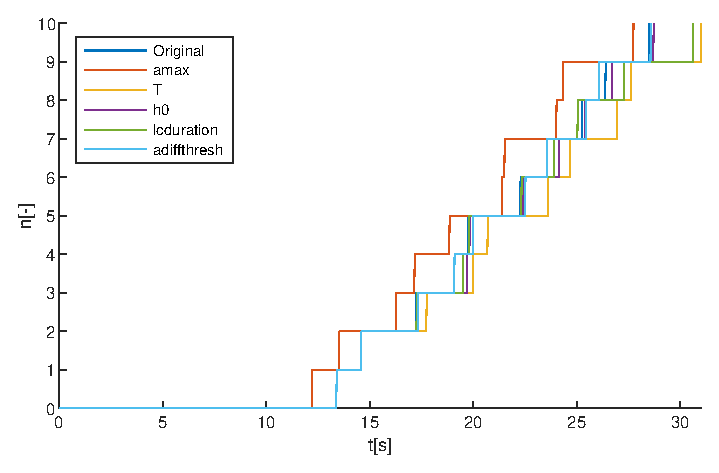
\includegraphics[width=0.75\textwidth]{eemobil/vehicle_density_par_pos_case1}
			\caption{Increasing the parameters with 25\% in case 1}
			\label{fig:vehicle_density_par_pos_case_1}
		\end{figure}
		\begin{table}[ht]
			\begin{center}
				\begin{tabular}{ |c|c|c|c|c|c|}
				\hline
				\vehicledensitypartable{1}
				\hline
				\end{tabular}
			\end{center}
			\caption{Increasing the parameters with 25\% in case 1}
			\label{tab:vehicle_density_par_pos_case_1}
		\end{table}
		
		The same analysis can be run on the different direction. Let us decrease the parameters by 25 \%. The effect can be seen in Table \ref{tab:vehicle_density_par_pos_case_2} and Figure \ref{fig:vehicle_density_par_pos_case_2}. The situation is exactly the opposite. Now $\amax$ has the greatest regression while $T$ has the greatest improvement on time.
		\begin{figure}[ht]
			\centering
			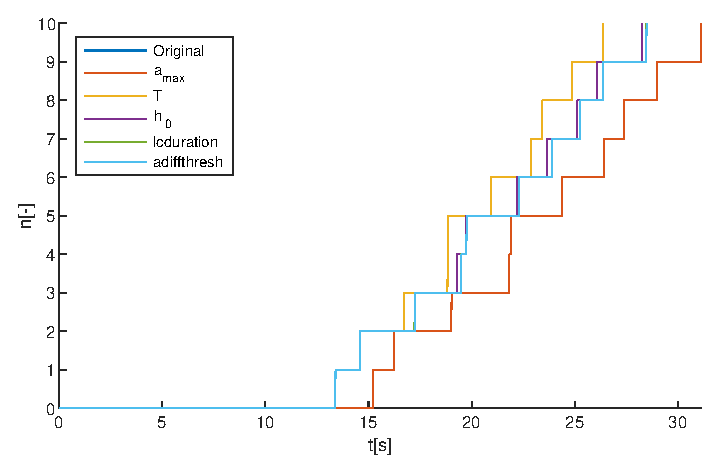
\includegraphics[width=0.75\textwidth]{eemobil/vehicle_density_par_pos_case2}
			\caption{Decreasing the parameters with 25\% in case 1}
			\label{fig:vehicle_density_par_pos_case_2}
		\end{figure}
		\begin{table}[ht]
			\begin{center}
				\begin{tabular}{ |c|c|c|c|c|c|}
				\hline
				\vehicledensitypartable{2}
				\hline
				\end{tabular}
			\end{center}
			\caption{Decreasing the parameters with 25\% in case 1}
			\label{tab:vehicle_density_par_pos_case_2}
		\end{table}
		\subsection{Changing parameters of case 2}
		Let us examine the other case as well. The expectation is that the parameters effect will be the same as for the previous case. First increase the value of the parameters then decrease by 25 \%. The results can be see on Table \ref{tab:vehicle_density_par_pos_case_3}, \ref{tab:vehicle_density_par_pos_case_4} and Figure \ref{fig:vehicle_density_par_pos_case_3}, \ref{fig:vehicle_density_par_pos_case_4}. The results show that only one parameter, the duration of lane change could improve the traffic flow in this case. This is understandable since there are almost three times more lane changes in case 2 then in case 1. However it is interesting to see that even with the increased $\amax$ value the final duration will be greater. On Figure \ref{fig:vehicle_density_par_pos_case_3} it is clear that for the first half of the simulation the increased $\amax$ improves the traffic flow then a lot of lane changes happened and the increased acceleration parameter turned out to be a drawback. A similar phenomena can be experienced on the congested highway traffic. In rush our it is common that the speed limit is lower then usual to avoid traffic jams.
		\begin{figure}
			\centering
			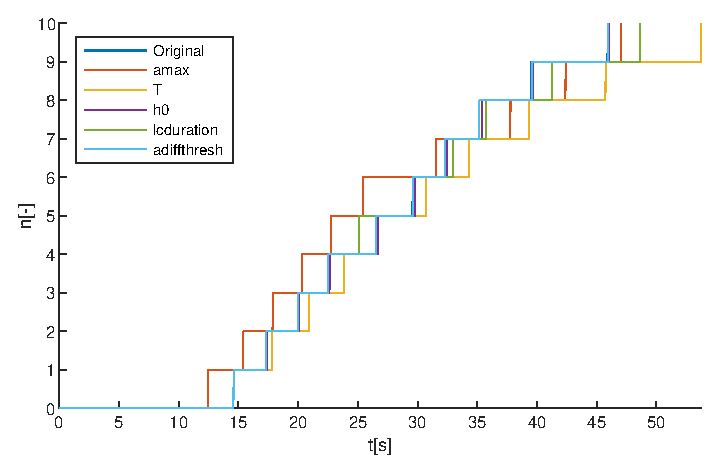
\includegraphics[width=0.75\textwidth]{eemobil/vehicle_density_par_pos_case3}
			\caption{Increasing the parameters with 25\% in case 2}
			\label{fig:vehicle_density_par_pos_case_3}
		\end{figure}
		\begin{table}
			\begin{center}
				\begin{tabular}{ |c|c|c|c|c|c|}
				\hline
				\vehicledensitypartable{3}
				\hline
				\end{tabular}
			\end{center}
			\caption{Increasing the parameters with 25\% in case 2}
			\label{tab:vehicle_density_par_pos_case_3}
		\end{table}
		\begin{figure}
			\centering
			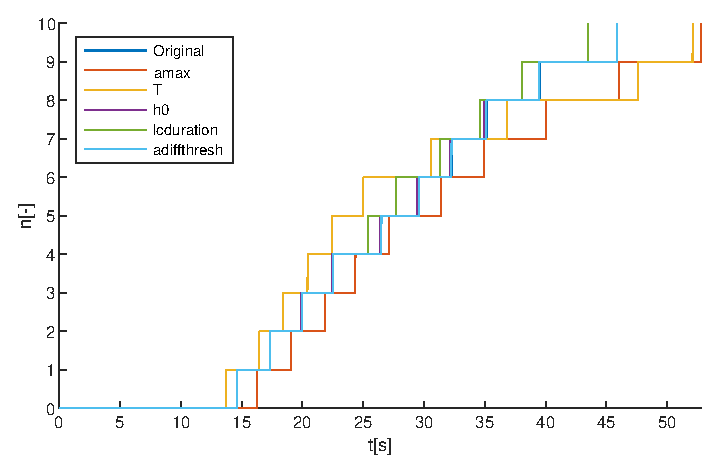
\includegraphics[width=0.75\textwidth]{eemobil/vehicle_density_par_pos_case4}
			\caption{Decreasing the parameters with 25\% in case 2}
			\label{fig:vehicle_density_par_pos_case_4}
		\end{figure}
		\begin{table}
			\begin{center}
				\begin{tabular}{ |c|c|c|c|c|c|}
				\hline
				\vehicledensitypartable{4}
				\hline
				\end{tabular}
			\end{center}
			\caption{Decreasing the parameters with 25\% in case 2}
			\label{tab:vehicle_density_par_pos_case_4}
		\end{table}
	\section{Model of a self-driving car}
		Nowadays almost every new car has some level of automated driving assistant feature. The automation level is scaled from 0 to 5 where 0 means the absolute human control and 5 means full autonomy. The low level automation like lane keeping or adaptive cruse control systems are quite common in today's car however nobody reached full autonomy yet. So why could an (half)autonomous car matter in a congested traffic. They may be better at deciding which lane to be in helping the every vehicles faster traveling. Another plus for the self-driving cars that they have a better reaction time than humans, and also they cannot be distracted from driving. These are just a few examples why a self-driving car could improve the capacity of a road network and make traffic better.

		So the task is to find a model for the autonomous driver. The key observation is that a self-driven car can be modeled with the same model as used before. The only difference relies on IDM and MOBIL parameters. So the task is to find proper parameters for the model that can be used for autonomous driver simulation.
	
		There are three main components representing human behavior built in the model currently. The first one is the attention for driving. An autonomous driver always paying attention to the road. The other component is that a self-driving car can always pay attention to both longitudinal and transversal motions. They are not limited to longitudinal motion attention when they have a higher acceleration or deceleration value. The last but not least component that it can have more favorable IDM and MOBIL parameters than most of the non self-driving cars. E.g. an autonomous driver will always accelerate with the greatest possible value which is comfortable, they would not change lanes if the advantage they would get be marginal however would put others significantly worst position.
	\section{Self-driving car variations in case 1}
		To test the effect of autonomous drivers in traffic, the same red traffic light situation was implemented. However in this case one of the driver's parameters have been substituted with an autonomous driver parameters. The most representative figure of the result of this task is where the count of cars passed the target line - 100 meters - is illustrated as a function of time. 
		\subsection{Effect of 1 self-driving car}
		Cars one by one have been exchanged and then simulated with the reaming cars. So a total of ten simulations were run. The result can be seen on Figure \ref{fig:vehicle_density}.
		\begin{figure}
			\centering
			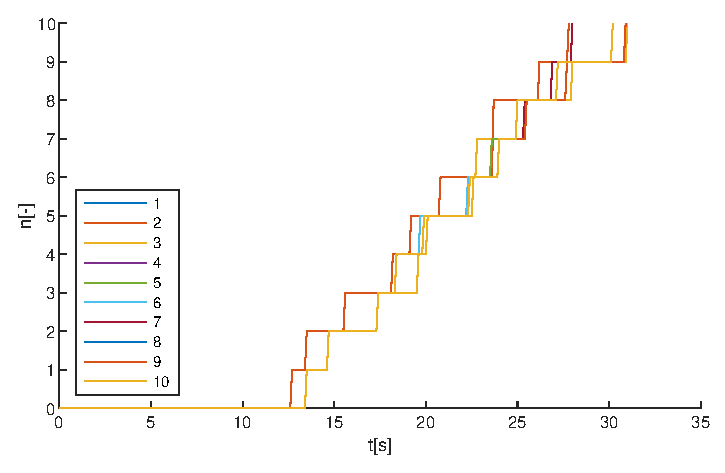
\includegraphics[width=0.75\textwidth]{eemobil/vehicle_density}
			\caption{Number of vehicles passes the target line with one self-driving car}
			\label{fig:vehicle_density}
		\end{figure}

		As Figure \ref{fig:vehicle_density} shows the first car reaches the target line in ~13 seconds. The interesting part is at the top right corner of the figure, where it can be seen that depending on which car has been exchanged the overall elapsed time can change up to 10 \%. The minimum, maximum, average and standard deviation values can be found in Table \ref{tab:vehicle_density_minmaxavg_case1}.
		\begin{table}
			\begin{center}
				\begin{tabular}{ |c|c|c|c|}
					\hline
					\vehicledensitytable{1}
					\hline
				\end{tabular}
			\end{center}
			\caption{Time until the last car has reached the target line. 1 autonomous car}
			\label{tab:vehicle_density_minmaxavg_case1}
		\end{table}
		
		In the hope of a better figure the same simulation results are shown on Figure \ref{fig:vehicle_density_avg} with averaged representation. It is slightly better than previously.
		
		\begin{figure}
			\centering
			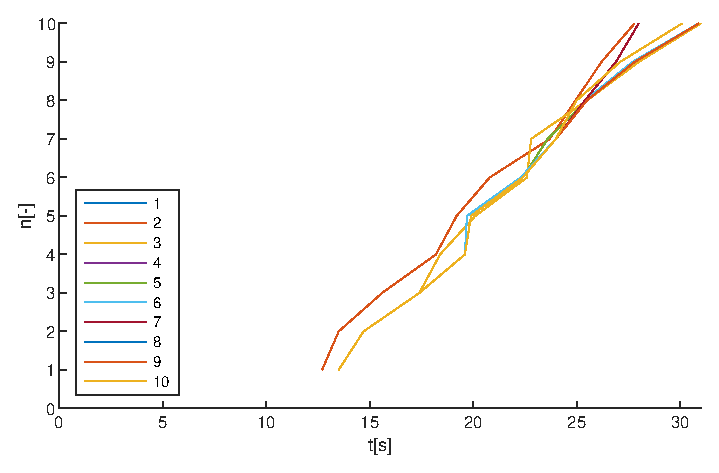
\includegraphics[width=0.75\textwidth]{eemobil/vehicle_density_avg}
			\caption{Number of vehicles passes the target line with one self-driving car}
			\label{fig:vehicle_density_avg}
		\end{figure}
		
		These simulations were run with only one self-driving car but in different positions. It can be seen that one autonomous driver could make the traffic faster. Based on the position of that one car most of the time it will decrease the overall duration.
		\subsection{Effect of 2 self-driving cars}
		Let us try the same simulation but this time run it exchanging two drivers to autonomous driver and see how the situation will improve. The total number of simulation was 45. All unique combinations were simulated. Figure \ref{fig:vehicle_density_case_2} and Table \ref{tab:vehicle_density_minmaxavg_case2} show the result.
		It can be seen that the minimum duration has decreased further.
		\begin{table}
			\begin{center}
				\begin{tabular}{ |c|c|c|c|}
					\hline
					\vehicledensitytable{2}
					\hline
				\end{tabular}
			\end{center}
			\caption{Time until the last car has reached the target line with two autonomous car}
			\label{tab:vehicle_density_minmaxavg_case2}
		\end{table}
		\begin{figure}
			\centering
			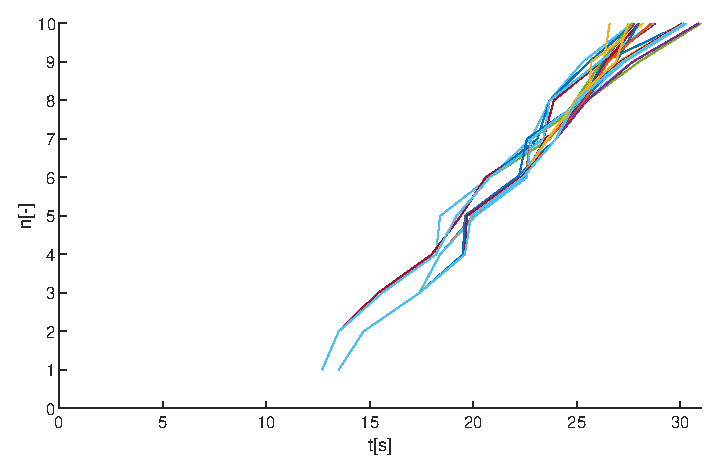
\includegraphics[width=0.75\textwidth]{eemobil/vehicle_density_case_2}
			\caption{Number of vehicles passes the target line with two self-driving cars}
			\label{fig:vehicle_density_case_2}
		\end{figure}

		\subsection{Effect of 3 self-driving cars}
		The same simulations were run with three self-driving cars as well. The total number of 120 unique combinations were simulated. Figure \ref{fig:vehicle_density_case_2} and Table \ref{tab:vehicle_density_minmaxavg_case2} show the result.
		\begin{table}
			\begin{center}
				\begin{tabular}{ |c|c|c|c|}
					\hline
					\vehicledensitytable{3}
					\hline
				\end{tabular}
			\end{center}
			\caption{Time until the last car has reached the target line with three autonomous car}
			\label{tab:vehicle_density_minmaxavg_case3}
		\end{table}
		\begin{figure}
			\centering
			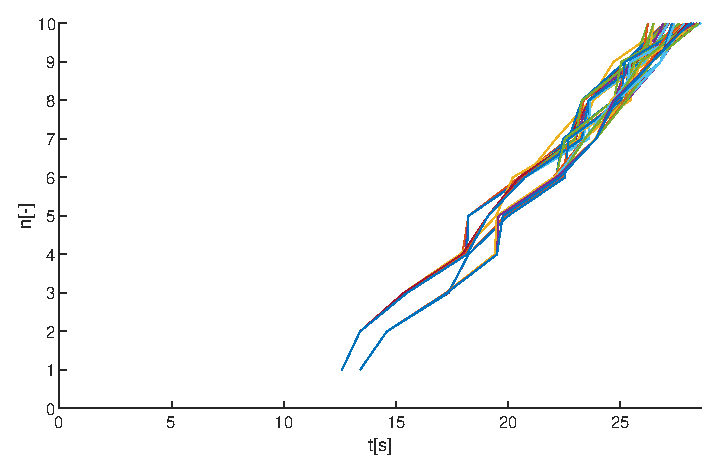
\includegraphics[width=0.75\textwidth]{eemobil/vehicle_density_case_3}
			\caption{Number of vehicles passes the target line with three self-driving cars}
			\label{fig:vehicle_density_case_3}
		\end{figure}
		\subsection{Analyzing all of the combinations}
		As seen in the previous examples the more self-driving vehicles are in the traffic the better the traffic flow is. So let us investigate all possible combinations to see what is the connection between the time and the number of self-driving cars. The expectation is that until a certain point the connection is almost linear but after that point self-driving cars cannot make traffic situation better.
		So all the possible combinations were simulated from only one exchanged car until all the ten cars exchanged. Table \ref{tab:all_variations} shows the count of the simulations for each exchanged car numbers.
		\begin{table}[ht]
			\begin{center}
				\begin{tabular}{ |c||c|c|c|c|c|c|c|c|c|c| }
					\hline
					Cars exchanged & 1   & 2    & 3    & 4     & 5      & 6     & 7     & 8   & 9   & 10\\
					\hline
					Variations            & 10 & 45 & 120 & 210 & 252 & 210 & 120 & 45 & 10 & 1\\
					\hline
				\end{tabular}
			\end{center}
			\caption{Number of variations}
			\label{tab:all_variations}
		\end{table}
		\begin{figure}
			\centering
			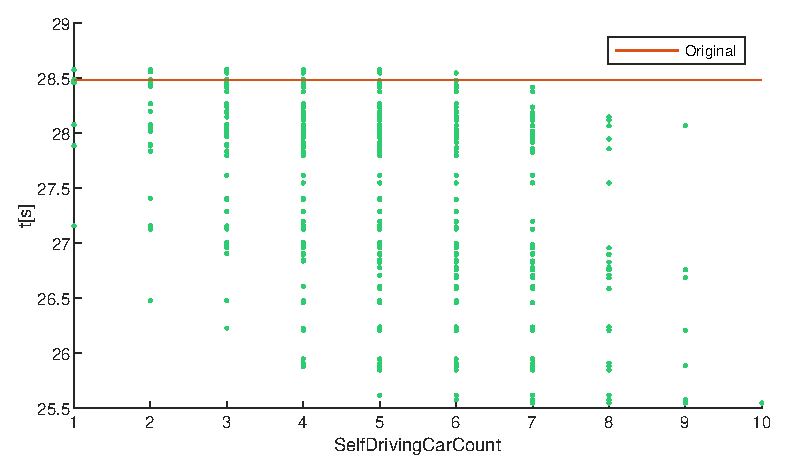
\includegraphics[width=0.8\textwidth]{eemobil/variations_nosize}
			\caption{Variation of autonomous drivers}
			\label{fig:self_variations_nosize}
		\end{figure}

		The result can be seen on Figure \ref{fig:self_variations_nosize}. The horizontal axis represents how many car has been exchanged. The vertical axis shows the duration of the simulation. The red line represents the original elapsed time without autonomous vehicles. Unfortunately most of the points are in the same place - because of the time step - so the figure could be a little bit misleading. To make it more expressive the plot has been modified to show a larger dot where there are more simulation results and smaller where there are just a few. The result of this modification can be seen on Figure \ref{fig:self_variations}. Figures \ref{fig:self_variations_avgminmax} and \ref{fig:self_variations_std} show the average, minimum, maximum and standard deviation for the simulations.
		
		As the plot shows the vast majority of dots are below the red line. It means that exchanging human driven cars to autonomous vehicles has an effect on the elapsed time, moreover this effect is positive since the time until the last car has reached the target line decreased. Interesting part of Figure \ref{fig:self_variations} is that at $t=27.5\rm s$ there are clearly visible gaps. After some investigation it turned out that above the gap there are only results when Vehicle 2 and Vehicle 7 stayed human driven and below the gap they are always autonomous vehicles.
		\begin{figure}
			\centering
			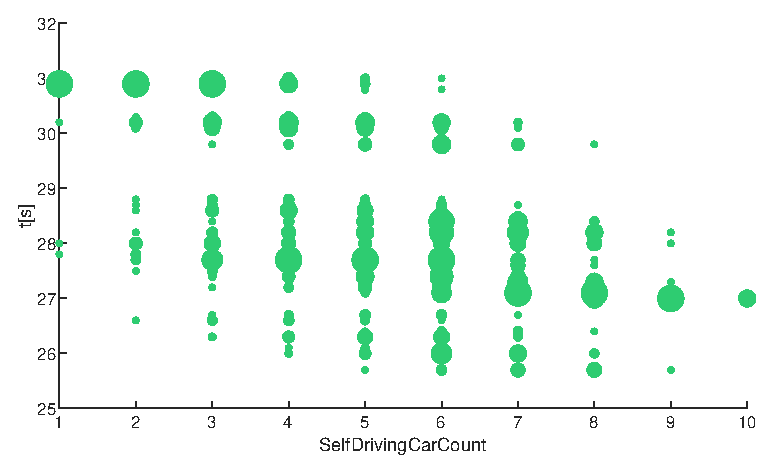
\includegraphics[width=0.8\textwidth]{eemobil/variations}
			\caption{Variation of autonomous drivers with highlights}
			\label{fig:self_variations}
		\end{figure}
		\begin{figure}
			\centering
			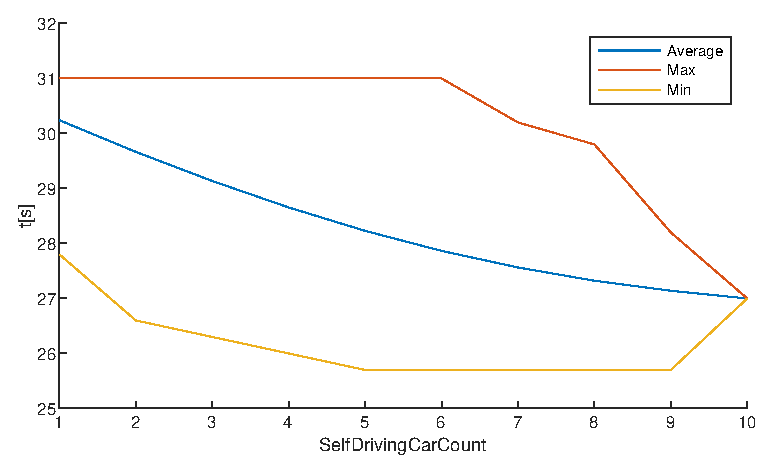
\includegraphics[width=0.8\textwidth]{eemobil/variations_avgminmax}
			\caption{Average, minimum and maximum of elapsed time.}
			\label{fig:self_variations_avgminmax}
		\end{figure}
		
		\begin{figure}
			\centering
			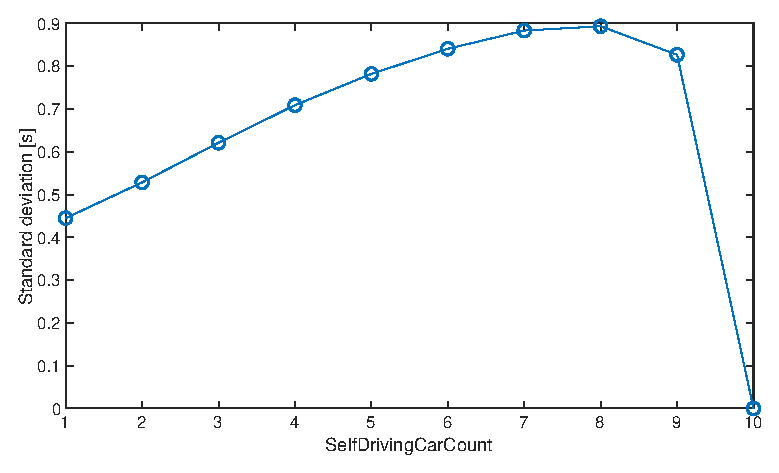
\includegraphics[width=0.8\textwidth]{eemobil/variations_std}
			\caption{Standard deviation of elapsed time}
			\label{fig:self_variations_std}
		\end{figure}
	\section{Self-driving car variations in case 2}
		Let us analyze the other case where the target line was 100 meters also, but there was an obstacle just before the line. The first three simulations can be skipped since unfortunately the result plots had no more meaningful than the plot containing all of the result. The same three plots were created for this case as well. In this case the self-driving cars are not performing that well as in case 1.
		\begin{figure}
			\centering
			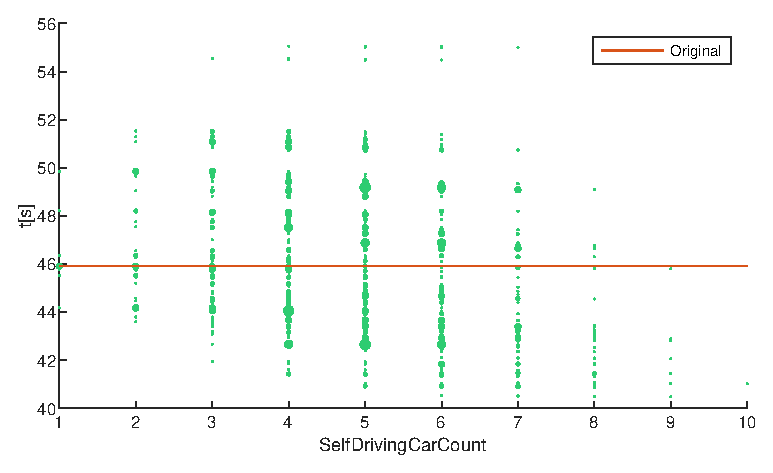
\includegraphics[width=0.8\textwidth]{eemobil/variations2}
			\caption{Time variation of autonomous drivers}
			\label{fig:self_variations2}
		\end{figure}
		\begin{figure}
			\centering
			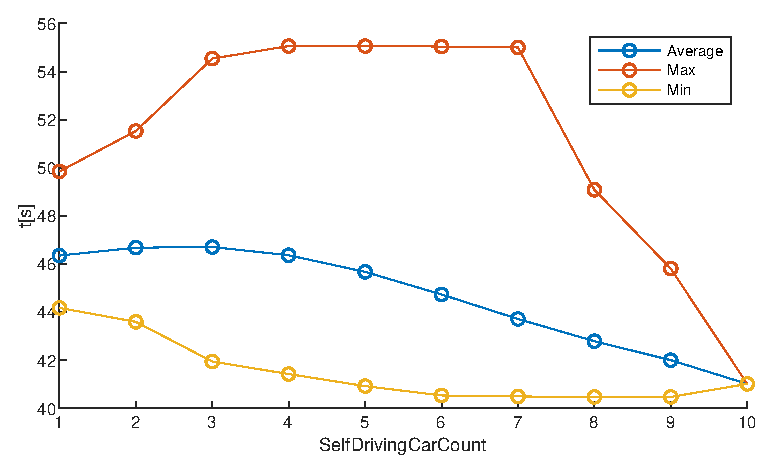
\includegraphics[width=0.8\textwidth]{eemobil/variations_avgminmax2}
			\caption{Average, minimum and maximum of elapsed time.}
			\label{fig:self_variations_avgminmax2}
		\end{figure}
		\begin{figure}
			\centering
			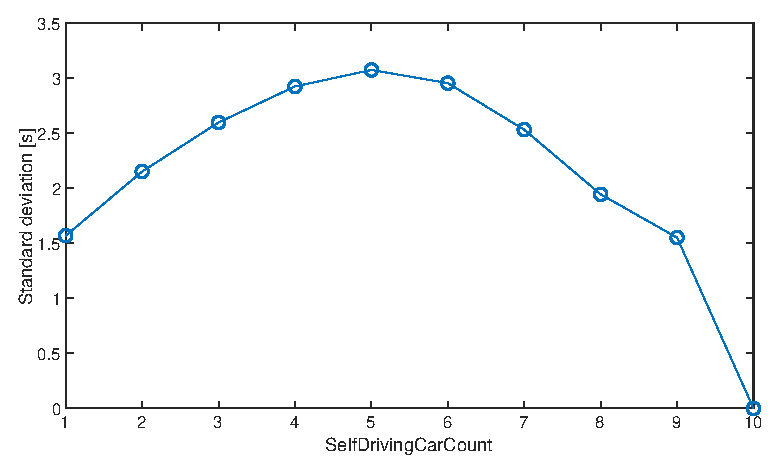
\includegraphics[width=0.8\textwidth]{eemobil/variations_std2}
			\caption{Standard deviation of elapsed time}
			\label{fig:self_variations_std2}
		\end{figure}
	\section{Conclusion}
		As a conclusion it can be stated that improvement of driver or vehicle parameter will improve the traffic flow as well. However the biggest improvement can be accomplished by exchanging human driven cars to autonomous vehicles. There are some edge cases however when self-driving cars would not improve the traffic situation either.
